\documentclass[11pt,a4paper]{article}
\usepackage[margin=1.5cm]{geometry}
\usepackage[T1]{fontenc}
\usepackage{lmodern}
\usepackage{tikz}
\usetikzlibrary{arrows.meta,positioning,fit,calc,shapes.geometric}
\usepackage{booktabs,longtable,array}
\usepackage{float}
\usepackage{caption}
\usepackage{hyperref}
\hypersetup{colorlinks=true,linkcolor=blue,urlcolor=blue}
\tikzset{
	box/.style={draw, rounded corners=2pt, align=center, minimum height=9mm, minimum width=27mm, fill=blue!8},
	layer/.style={draw, rounded corners=3pt, align=center, minimum height=12mm, minimum width=36mm, fill=gray!10},
	store/.style={draw, cylinder, shape border rotate=90, aspect=0.25, align=center, minimum height=14mm, minimum width=30mm, fill=green!10},
	flow/.style={-{Latex[length=2mm]}, thick},
	event/.style={-{Latex[length=2mm]}, dashed, thick},
	note/.style={draw, rounded corners=2pt, align=left, fill=yellow!12, font=\small}
}
\title{System Design\\Real-Time Service Request Management System}
\author{}
\date{}
\begin{document}
\maketitle

\section{Architecture Overview}
The system is a decoupled, multi-tier application: a React presentation tier, an Express API tier, a Socket.IO real-time tier, a Worker Thread concurrency tier, and a MongoDB persistence tier.

The architecture and data flow are illustrated in the diagrams below.

\begin{figure}[H]
\centering
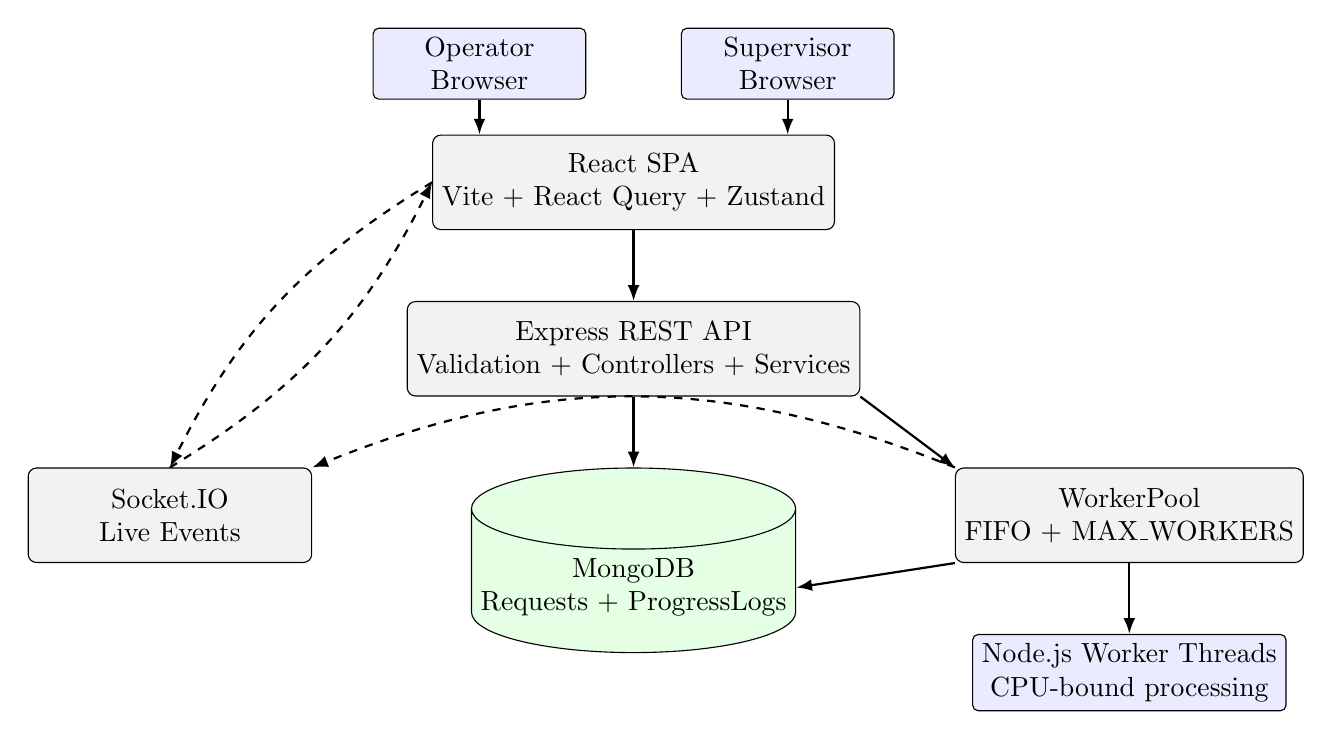
\begin{tikzpicture}[node distance=9mm and 12mm]
	\node[box] (operator) {Operator\\Browser};
	\node[box, right=of operator] (supervisor) {Supervisor\\Browser};
	\node[layer, below=of $(operator)!0.5!(supervisor)$] (frontend) {React SPA\\Vite + React Query + Zustand};
	\node[layer, below=of frontend] (api) {Express REST API\\Validation + Controllers + Services};
	\node[layer, below left=of api] (socket) {Socket.IO\\Live Events};
	\node[layer, below right=of api] (pool) {WorkerPool\\FIFO + MAX\_WORKERS};
	\node[box, below=of pool] (workers) {Node.js Worker Threads\\CPU-bound processing};
	\node[store, below=of api] (db) {MongoDB\\Requests + ProgressLogs};
	\draw[flow] (operator.south) -- (operator.south |- frontend.north);
	\draw[flow] (supervisor.south) -- (supervisor.south |- frontend.north);
	\draw[flow] (frontend.south) -- (api.north);
	\draw[event] (frontend.west) to[bend right=16] (socket.north);
	\draw[flow] (api.south east) -- (pool.north west);
	\draw[flow] (api.south) -- (db.north);
	\draw[flow] (pool.south) -- (workers.north);
	\draw[flow] (pool.south west) -- (db.east);
	\draw[event] (pool.north west) to[bend right=22] (socket.north east);
	\draw[event] (socket.north) to[bend right=16] (frontend.west);
\end{tikzpicture}
\caption{High-level architecture.}
\end{figure}

\section{Component Diagram}
The frontend consists of the request form, role-specific pages, reusable request cards, filters, detail modal, React Query API hooks, and the Socket.IO subscription hook. The backend follows Routes and Validation $\rightarrow$ Controllers $\rightarrow$ Services $\rightarrow$ Repositories $\rightarrow$ Mongoose Models. The Service layer dispatches work to the WorkerPool, while the WorkerPool runs the worker script and forwards progress to persistence and Socket.IO.

\begin{figure}[H]
\centering
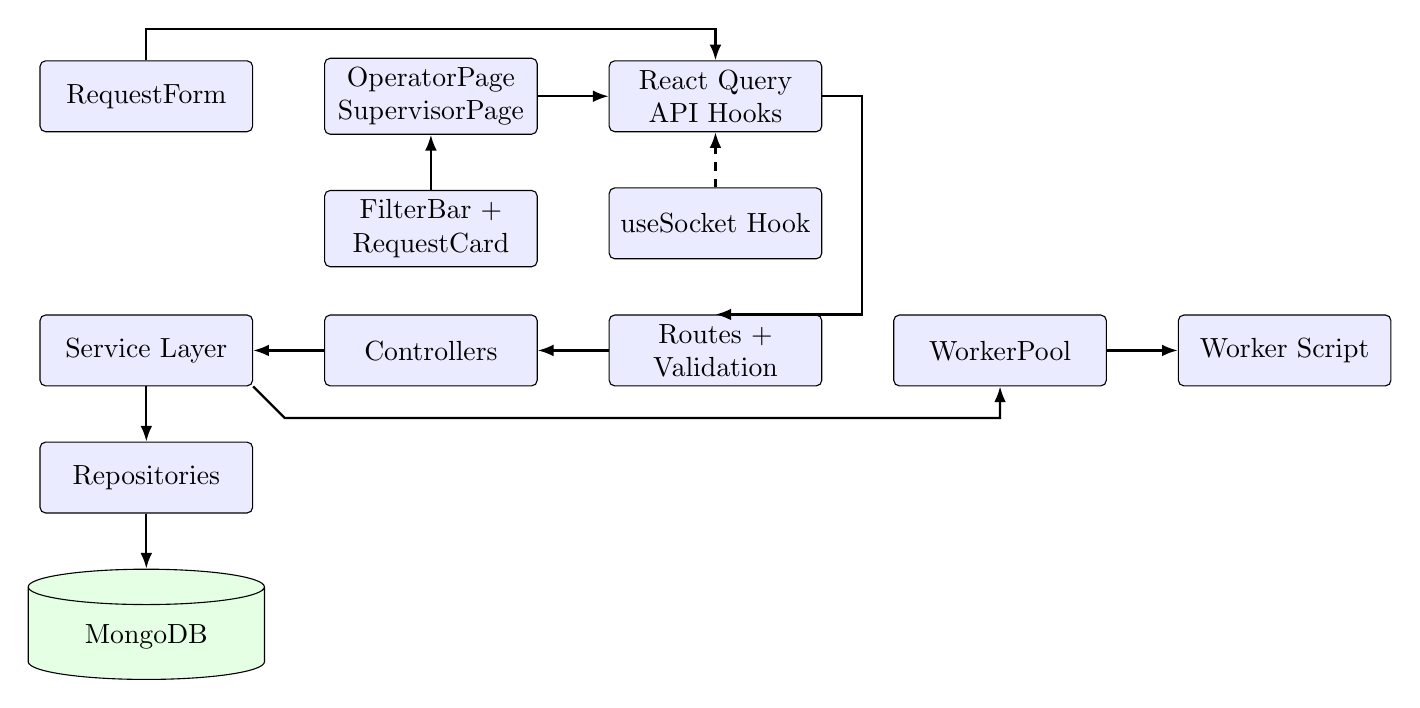
\begin{tikzpicture}[node distance=7mm and 9mm]
	\node[box] (form) {RequestForm};
	\node[box, right=of form] (pages) {OperatorPage\\SupervisorPage};
	\node[box, right=of pages] (query) {React Query\\API Hooks};
	\node[box, below=of pages] (filter) {FilterBar +\\RequestCard};
	\node[box, below=of query] (socketc) {useSocket Hook};
	\node[box, below=of socketc] (routes) {Routes +\\Validation};
	\node[box, left=of routes] (controller) {Controllers};
	\node[box, left=of controller] (service) {Service Layer};
	\node[box, below=of service] (repo) {Repositories};
	\node[box, right=of routes] (workerpool) {WorkerPool};
	\node[box, right=of workerpool] (worker) {Worker Script};
	\node[store, below=of repo] (database) {MongoDB};
	\draw[flow] (form.north) -- ++(0,4mm) -| (query.north);
	\draw[flow] (pages.east) -- (query.west);
	\draw[flow] (filter.north) -- (pages.south);
	\draw[event] (socketc.north) -- (query.south);
	\draw[flow] (query.east) -- ++(5mm,0) |- (routes.north);
	\draw[flow] (routes.west) -- (controller.east);
	\draw[flow] (controller.west) -- (service.east);
	\draw[flow] (service.south) -- (repo.north);
	\draw[flow] (repo.south) -- (database.north);
	\draw[flow] (service.south east) -- ++(4mm,-4mm) -| (workerpool.south);
	\draw[flow] (workerpool.east) -- (worker.west);
\end{tikzpicture}
\caption{Frontend and layered backend components.}
\end{figure}

\section{Database Design}
MongoDB contains two logical collections. \textbf{ServiceRequest} stores the request identity, title, description, priority, lifecycle status, progress percentage, current stage, submitter, and lifecycle timestamps. \textbf{ProgressLog} stores the parent request identifier, stage, message, progress percentage, and timestamp. One service request has many progress logs.

\begin{figure}[H]
\centering
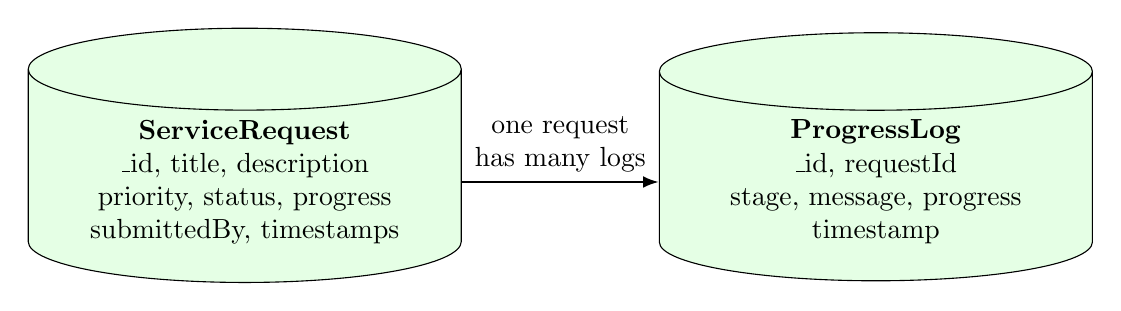
\begin{tikzpicture}[node distance=25mm]
	\node[store, minimum width=55mm, minimum height=25mm] (request) {\textbf{ServiceRequest}\\
		\_id, title, description\\
		priority, status, progress\\
		submittedBy, timestamps};
	\node[store, right=of request, minimum width=55mm, minimum height=25mm] (log) {\textbf{ProgressLog}\\
		\_id, requestId\\
		stage, message, progress\\
		timestamp};
	\draw[flow] (request.east) -- node[above, align=center] {one request\\has many logs} (log.west);
\end{tikzpicture}
\caption{MongoDB collections and logical relationship.}
\end{figure}

\section{API Design}
\begin{longtable}{p{0.12\textwidth}p{0.32\textwidth}p{0.42\textwidth}}
\toprule Method & Endpoint & Purpose\\\midrule
POST & /api/requests & Create and enqueue a request\\
GET & /api/requests & List with pagination, sorting, search, and filters\\
GET & /api/requests/:id & Retrieve one request\\
POST & /api/requests/:id/cancel & Cancel pending or processing request\\
GET & /api/requests/:id/progress & Retrieve progress audit logs\\
GET & /health & Health check\\
\bottomrule
\end{longtable}

\section{WebSocket Communication Flow}
The Operator submits through the REST API. The API emits \texttt{request:created} and enqueues the job. The WorkerPool emits status and progress events through Socket.IO as the worker advances. These events are pushed to connected Operator and Supervisor clients without polling. Events include \texttt{requests:initial-state}, \texttt{request:created}, \texttt{request:status-updated}, \texttt{request:progress-updated}, \texttt{request:completed}, \texttt{request:failed}, and \texttt{request:cancelled}.

\begin{figure}[H]
\centering
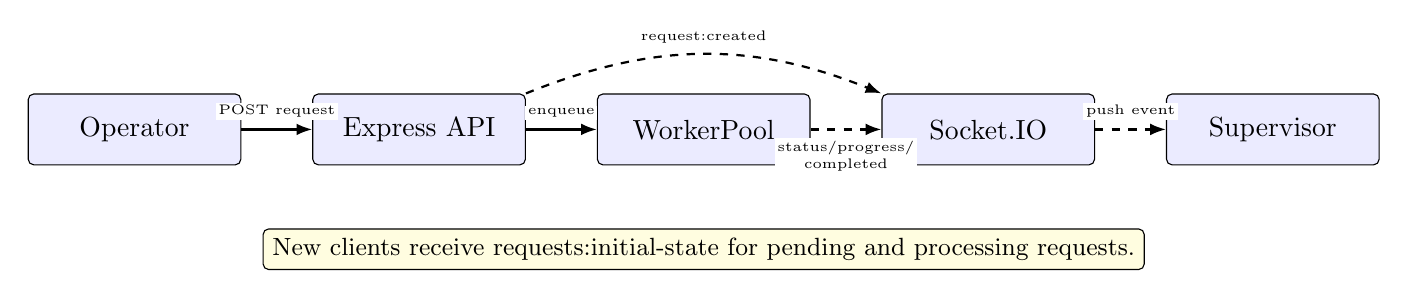
\begin{tikzpicture}[node distance=8mm and 9mm]
	\node[box] (op) {Operator};
	\node[box, right=of op] (api2) {Express API};
	\node[box, right=of api2] (pool2) {WorkerPool};
	\node[box, right=of pool2] (socket2) {Socket.IO};
	\node[box, right=of socket2] (sup) {Supervisor};
	\draw[flow] (op.east) -- node[above=1mm, fill=white, inner sep=1pt, font=\tiny] {POST request} (api2.west);
	\draw[flow] (api2.east) -- node[above=1mm, fill=white, inner sep=1pt, font=\tiny] {enqueue} (pool2.west);
	\draw[event] (api2.north east) to[bend left=22]
		node[above=1mm, fill=white, inner sep=1pt, font=\tiny] {request:created} (socket2.north west);
	\draw[event] (pool2.east) -- node[below=1mm, fill=white, inner sep=1pt, font=\tiny, align=center] {status/progress/\\completed} (socket2.west);
	\draw[event] (socket2.east) -- node[above=1mm, fill=white, inner sep=1pt, font=\tiny] {push event} (sup.west);
	\node[note, below=of pool2] {New clients receive requests:initial-state for pending and processing requests.};
\end{tikzpicture}
\caption{Server-pushed events without polling.}
\end{figure}

\section{Concurrency Model}
The WorkerPool defaults to five workers. Each worker performs six CPU-bound stages in 100 millisecond chunks, yields with \texttt{setImmediate}, and checks for cooperative cancellation. Workers communicate with the main thread through \texttt{parentPort}; only the main thread writes to MongoDB and broadcasts Socket.IO events.
Incoming jobs enter a FIFO queue. The dispatcher starts jobs while the active worker count is below \texttt{MAX\_WORKERS}; remaining jobs wait until a worker exits. The concurrency model is illustrated below.

\begin{figure}[H]
\centering
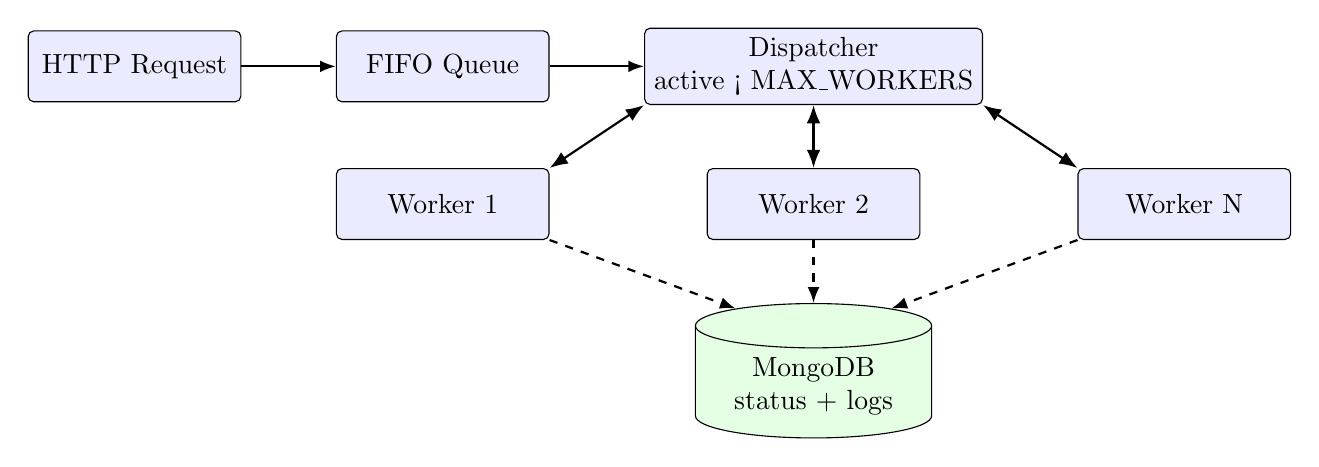
\begin{tikzpicture}[node distance=8mm and 12mm]
	\node[box] (ingest) {HTTP Request};
	\node[box, right=of ingest] (queue) {FIFO Queue};
	\node[box, right=of queue] (dispatch) {Dispatcher\\active < MAX\_WORKERS};
	\node[box, below left=of dispatch] (w1) {Worker 1};
	\node[box, below=of dispatch] (w2) {Worker 2};
	\node[box, below right=of dispatch] (wn) {Worker N};
	\node[store, below=of w2] (db2) {MongoDB\\status + logs};
	\draw[flow] (ingest.east) -- (queue.west);
	\draw[flow] (queue.east) -- (dispatch.west);
	\draw[Latex-Latex, thick] (dispatch.south west) -- (w1.north east);
	\draw[Latex-Latex, thick] (dispatch.south) -- (w2.north);
	\draw[Latex-Latex, thick] (dispatch.south east) -- (wn.north west);
	\draw[event] (w1.south east) -- (db2.north west);
	\draw[event] (w2.south) -- (db2.north);
	\draw[event] (wn.south west) -- (db2.north east);
\end{tikzpicture}
\caption{Bounded Worker Thread execution with queued overflow.}
\end{figure}

\section{Technology Justification}
React and TypeScript provide a component-based, type-safe UI. Vite provides fast development builds. TanStack Query manages server state and cache updates, while Zustand manages the role workspace. Express and Node.js provide non-blocking HTTP and WebSocket handling. Socket.IO provides reliable event delivery and reconnection. Node.js \texttt{worker\_threads} isolate CPU-bound work. MongoDB and Mongoose provide persistence, indexes, and schema constraints. Zod provides declarative validation. Vitest, Supertest, and MongoMemoryServer provide isolated API tests.

\section{Security and Trade-offs}
CORS, rate limiting, Zod validation, and production error obfuscation are implemented. Authentication and backend RBAC are future enhancements. The in-process FIFO queue avoids Redis infrastructure but limits horizontal scaling to a single server node.
\end{document}
